% !TeX program = pdflatex
% !TeX root = main.tex
% IEEE conference format; wording, results and figures follow reportdraft.en.md.
\documentclass[conference,a4paper]{IEEEtran}
\usepackage[T1]{fontenc}
\usepackage{cite}
\usepackage{amsmath,amssymb}
\usepackage{graphicx}
\usepackage{booktabs,tabularx,array}
\usepackage[hidelinks]{hyperref}
\usepackage{url}
\usepackage{placeins}
\graphicspath{{images/}{figures/}}
\setlength{\emergencystretch}{1em}
\newcommand{\authornames}{Hongze Li \quad and \quad Jiatong Wu}
\newcommand{\studentids}{Student IDs: 1820462 \quad and \quad 1822875}
\title{Evaluating Global and Local Visual Features for House Price Prediction}
\author{\IEEEauthorblockN{\authornames}
\IEEEauthorblockA{\studentids\\
COMP90086 Computer Vision, The University of Melbourne}}
\hypersetup{pdftitle={Evaluating Global and Local Visual Features for House Price Prediction},pdfauthor={Hongze Li and Jiatong Wu}}
\begin{document}
\maketitle
\raggedbottom
% No abstract or keywords, following the report's established writing brief.
% !TeX root = ../main.tex

\section{Introduction}

% Typeset from reportdraft.en.md; edit this TeX file for subsequent revisions.

A very important step in putting a property on the market is setting a reasonable price, and real estate agents usually combine property characteristics, market conditions and information on comparable transactions to recommend a listing price \cite{nar2026pricing}. A reasonable valuation can provide an agency with a good starting point for negotiation, and can also help real estate platforms determine which properties need further price review. Although these potential uses reflect the practical value of house price prediction, estimating a price from a single image is still difficult. A photograph can contain information on architectural style, the visible extent of the building and the surrounding environment, but does not directly provide the floor area, precise location or interior condition. At the same time, different viewing angles, lighting and occlusion of the same house can also affect the estimation of its price.

In this project, we used 8,000 images with price labels, drawn from a Southern California real-estate listing dataset \cite{dogan2019socal}, to train lightweight regressors on frozen pretrained visual features, to accommodate limited labels and compute. During model training, we focused on studying whether combining whole-image and local features could reduce prediction error and whether price-order auxiliary supervision could further improve prediction. Finally, we further combined the relevant experimental models to investigate whether using different models together would increase prediction accuracy.

% !TeX root = ../main.tex

\section{Method}


\begin{table}[!htbp]
\centering\footnotesize
\caption{Training objective and notation}
\label{tab:objective}
\begin{tabularx}{\linewidth}{@{}>{\raggedright\arraybackslash}p{0.15\linewidth}>{\raggedright\arraybackslash}p{0.25\linewidth}>{\raggedright\arraybackslash}X@{}}
\toprule
Symbol & Meaning & Calculation or value used in this project \\
\midrule
\(\mathcal{L}\) & Total training loss & Sum of the price prediction loss and the weighted auxiliary loss \\
\(\mathcal{L}_{\mathrm{price}}\) & Price prediction loss & Mean squared error of standardised log(price) \\
\(\mathcal{L}_{\mathrm{order}}\) & Auxiliary loss for the four price-threshold judgements & Binary cross-entropy for the four binary judgements, averaged over samples and thresholds \\
\(\lambda\) & Weight of the auxiliary loss & 0.3 in the combined experiments; 0 for regression only \\
\bottomrule
\end{tabularx}

\end{table}

\begin{table*}[!t]
\centering\footnotesize
\caption{Regression and post-processing configuration}
\label{tab:configuration}
\begin{tabularx}{\linewidth}{@{}>{\raggedright\arraybackslash}p{0.18\linewidth}>{\raggedright\arraybackslash}X@{}}
\toprule
Setting & Configuration used in this project \\
\midrule
Network structure & Two hidden layers with widths of 512 and 256; each layer uses BatchNorm, GELU and dropout (0.3) \\
Output & 1 scalar for regression only; adding ordinal supervision introduces 4 additional threshold judgements, while the final valuation still uses only the scalar output \\
Optimiser & AdamW; weight decay 0.01 \\
Learning rate schedule & OneCycle; maximum learning rate 0.001, with the first 15\% of scheduling steps used to increase the learning rate \\
Training budget & Each regression head is trained for 40 epochs, with 256 samples per batch \\
Auxiliary thresholds & The 20\%, 40\%, 60\% and 80\% price quantiles of the corresponding training portion \\
Individual predictor calibration & Within each outer training portion, ordinary random five-fold splits generate held-out predictions; these predictions and the training labels are used to fit an isotonic correction curve, which is then applied to the outer validation predictions \\
Ensemble and output range & The nine predictors use non-negative least-squares weights, followed by linear correction; final predictions are limited to 195--2,000 thousand dollars \\
\bottomrule
\end{tabularx}

\end{table*}

\begin{table}[!htbp]
\centering\footnotesize
\caption{Inputs to the nine ensemble members}
\label{tab:members}
\begin{tabularx}{\linewidth}{@{}>{\raggedright\arraybackslash}p{0.12\linewidth}>{\raggedright\arraybackslash}X>{\centering\arraybackslash}p{0.15\linewidth}@{}}
\toprule
Predictor & Input feature groups & Number of feature groups \\
\midrule
P1 & H+@336 + H+@256 + L@336 + D2L@336 + T + M & 6 \\
P2 & H+@336 + L@336 + M & 3 \\
P3 & H+@336 + L@336 + T + M & 4 \\
P4 & H+@224 + H+@336 & 2 \\
P5 & H+@336 & 1 \\
P6 & H+@256 & 1 \\
P7 & L@336 & 1 \\
P8 & T & 1 \\
P9 & D2L@518 & 1 \\
\bottomrule
\end{tabularx}

\par\smallskip{\footnotesize\raggedright\textit{Note:} H+ and L denote DINOv3 ViT-H+ and ViT-L, respectively, and D2L denotes DINOv2 ViT-L; @s denotes an s\ensuremath{\times}s-pixel input. T is the mean of the features from the 2\ensuremath{\times}2 local tiles extracted using L@224; M consists of 19 image statistics (such as dimensions and sharpness).\par}
\end{table}

% Typeset from reportdraft.en.md; edit this TeX file for subsequent revisions.

Our overall idea is to first convert images into numerical features and then learn the relationship between these features and house prices. We first resized all images to the specified square input size, then used the DINOv3 \cite{simeoni2025dinov3} image model with frozen parameters to extract features, and trained a small regression network using price labels. To test whether local views could provide additional information, we separately processed the full image and the four non-overlapping local tiles obtained by dividing the original image evenly into a 2\ensuremath{\times}2 grid. Each image tile was resized and its features were extracted separately, and the four groups of features were then averaged and concatenated with the whole-image features before being fed into the regression network. We then used controlled experiments to evaluate whether this whole-image + local combination was better than using only the whole image.

For price prediction, we used a small neural network (MLP). The input features were first standardised using statistics from the training portion; the target prices were also first log-transformed and standardised to put them on a more concentrated numerical scale, and the predictions were then transformed back into prices. We also studied an auxiliary task that asked the network to judge whether the house price was greater than four price thresholds at the same time (these thresholds were determined from the price distribution in the corresponding training portion, dividing the houses into five groups with approximately equal numbers). Therefore, while the network was learning specific numerical values, it was also learning the ordering of prices from low to high. The training objective consists of the price prediction error and the error in judging price order, with the parameter \ensuremath{\lambda} controlling the weight of the auxiliary task. The two tasks share the regression network, but the final valuation only uses the price prediction output. All results are evaluated on the original price scale after the inverse transformation.

\[
\mathcal{L}=\mathcal{L}_{\mathrm{price}}+\lambda\mathcal{L}_{\mathrm{order}}.
\]


After the above price prediction, we further calibrated it, using a correction curve to adjust the predicted values to bring them closer to the actual prices, and then applied the curve to the validation samples. Apart from adjusting the output of an individual predictor, we also studied whether different predictors were complementary, namely how different visual features, input sizes and local views would produce different prediction errors. To further study the effect of combining different image information, we added frozen DINOv2 \cite{oquab2024dinov2} features alongside DINOv3, and examined combinations of whole-image features at different input sizes, local features, and image statistics such as image dimensions and sharpness. Each feature configuration was used to train a separate MLP price predictor, with the specific compositions shown in Table~\ref{tab:members}. We combined the outputs of nine existing regression predictors using weights, and then applied an overall linear correction to the combined result. We divided the data into five parts and took turns using one part to evaluate the ensemble. Each time, we used the existing predicted prices and true prices from the other four parts to determine the ensemble weights and overall correction parameters, and then applied these parameters to the currently held-out part. The specific regression network structure, training parameters and post-processing settings are shown in Table~\ref{tab:configuration}.



% !TeX root = ../main.tex

\section{Experiments and Results}


\begin{table}[!htbp]
\centering\footnotesize
\caption{Regressor and image-view comparisons}
\label{tab:comparisons}
\textbf{(a) Regressors with identical frozen features}\par\smallskip
\begin{tabularx}{\linewidth}{@{}>{\raggedright\arraybackslash}X r@{}}
\toprule
Regressor & OOF MSE \ensuremath{\downarrow} \\
\midrule
MLP & \textbf{70,818} \\
Ridge & 72,624 \\
XGBoost & 74,140 \\
\bottomrule
\end{tabularx}

\par\smallskip{\footnotesize\raggedright\textit{Note:} All three use whole-image features extracted by DINOv3 ViT-H+ from 336\ensuremath{\times}336-pixel inputs and the same fixed grouped five-fold split, with detected near-duplicate images kept in the same fold. The following result tables all report OOF MSE on the original price scale, in (thousand dollars)², rounded to integers.\par}
\medskip
\textbf{(b) Whole-image and local views with the same encoder}\par\smallskip
\begin{tabularx}{\linewidth}{@{}>{\raggedright\arraybackslash}X r@{}}
\toprule
Input features & OOF MSE \ensuremath{\downarrow} \\
\midrule
Whole image & 76,802 \\
Mean features from 2\ensuremath{\times}2 local tiles & 76,800 \\
Concatenated whole-image and local features & \textbf{74,936} \\
\bottomrule
\end{tabularx}

\par\smallskip{\footnotesize\raggedright\textit{Note:} Both the whole image and each local tile use DINOv3 ViT-L with 224\ensuremath{\times}224-pixel inputs; all regressors are regression-only MLPs. The three rows use the same evaluation split, and concatenation reduces MSE by approximately 2.4\% relative to the whole image. These are single-seed results.\par}
\end{table}

\begin{table}[!htbp]
\centering\footnotesize
\caption{Local features and ordinal supervision}
\label{tab:ordinal}
\begin{tabularx}{\linewidth}{@{}>{\raggedright\arraybackslash}X>{\centering\arraybackslash}p{0.24\linewidth}>{\centering\arraybackslash}p{0.24\linewidth}@{}}
\toprule
Input configuration & Continuous regression only (\ensuremath{\lambda}=0) & Continuous regression + ordinal (\ensuremath{\lambda}=0.3) \\
\midrule
Global DINOv3 ViT-H+@336 & 70,818 & 70,722 \\
Global DINOv3 ViT-H+@336 + local DINOv3 ViT-L@224 & \textbf{70,236} & 70,367 \\
\bottomrule
\end{tabularx}

\par\smallskip{\footnotesize\raggedright\textit{Note:} Values are OOF MSE in (thousand dollars)². Local features are the mean features of the four tiles in a 2\ensuremath{\times}2 grid. The global and local branches use different encoders and input sizes, so this comparison concerns the complete configuration with this local branch added; the view comparison using the same encoder is shown in Table~\ref{tab:comparisons}(b). All four settings have single-seed results, and the small differences have not undergone complete repeated validation.\par}
\end{table}

\begin{table*}[!t]
\centering\footnotesize
\caption{Feature combination and prediction averaging}
\label{tab:ensemble}
\begin{tabularx}{\linewidth}{@{}>{\raggedright\arraybackslash}p{0.28\linewidth}>{\raggedright\arraybackslash}X r@{}}
\toprule
Configuration & What is combined and how it is trained & OOF MSE \ensuremath{\downarrow} \\
\midrule
Six concatenated feature groups + MLP & P1 in Table~\ref{tab:members}; one random initialisation & 69,175 \\
Same six-group configuration, prediction averaging over three seeds & P1 trained with three different random initialisations, followed by averaging the price predictions & 68,522 \\
Nine-member prediction ensemble & P1--P9 in Table~\ref{tab:members}; non-negative least-squares weights + linear correction & \textbf{65,278} \\
\bottomrule
\end{tabularx}

\par\smallskip{\footnotesize\raggedright\textit{Note:} MSE is in (thousand dollars)². The approximately 5.6\% reduction uses 69,175 as the comparison baseline. The nine-member ensemble uses the single-seed predictions of each member, rather than directly adding members to the three-seed average; the three rows also do not form a complete ablation that changes only one factor. The value of 65,278 is a local development OOF estimate; member selection and the overall process have not been fully independently validated, and it is not a measured Kaggle score.\par}
\end{table*}

% Typeset from reportdraft.en.md; edit this TeX file for subsequent revisions.

We compare price prediction methods, image inputs, the auxiliary task and prediction combinations under one controlled setting: a fixed five-group split that keeps the price distribution of each part similar, evaluated by mean squared error (MSE), where lower is better. We first tested three price prediction methods: MLP, Ridge and XGBoost \cite{chen2016xgboost}. All three used the same DINOv3 ViT-H+ image features extracted using 336\ensuremath{\times}336-pixel inputs. Table~\ref{tab:comparisons}(a) shows that the MSEs of MLP, Ridge and XGBoost were 70,818, 72,624 and 74,140, respectively, with MLP having the lowest error in the tested settings. The subsequent comparisons therefore all used MLP, so that image input and the auxiliary task could be varied against a fixed regressor.


The image encoder was also chosen by comparison. Holding the regressor and the split fixed, replacing supervised ImageNet-22k pretraining with self-supervised DINOv3 pretraining on the same ConvNeXt-B architecture lowered the MSE from 98,752 to 87,744, and exchanging ConvNeXt-L for ViT-L under the same DINOv3 pretraining lowered it from 86,454 to 76,802, both by about 11\%. Doubling capacity from ConvNeXt-B to ConvNeXt-L under fixed pretraining was worth only 1.5\%. A plausible reason is that every image here shows the same object class, so the invariances that help a classifier separate categories also discard the within-class appearance variation price depends on.


After fixing the price prediction method, we next checked whether using full photographs, local images or a combination of the two would affect the results. To keep the image model consistent in this view comparison, both whole-image and local features were extracted using DINOv3 ViT-L with 224\ensuremath{\times}224-pixel inputs. The MSEs of using only the whole image and only local features were almost the same, at 76,802 and 76,800, respectively; concatenating the two groups of features reduced the MSE to 74,936, approximately 2.4\% lower than using the whole image (Table~\ref{tab:comparisons}(b)). In this configuration local features therefore supplement whole-image information rather than replacing it.

Besides testing different combinations of views, we also examined whether the auxiliary task of judging higher or lower prices (ordinal) could improve prediction. Using the lower-error ViT-H+ whole-image configuration at 336\ensuremath{\times}336 pixels, we varied whether ViT-L@224 local features were added and whether the auxiliary task was enabled (Table~\ref{tab:ordinal}). The results show that the auxiliary task itself only slightly reduced the error of the whole-image configuration, while slightly increasing it when whole-image and local features were combined. Because the changes were small and inconsistent in direction, we cannot determine whether the price-order auxiliary task can provide a stable additional benefit.


Finally, we also tried some combinations of different strategies (Table~\ref{tab:ensemble}), concatenating six groups of features and feeding them into the same MLP, which gave an MSE of 69,175; training the same configuration with three different random initialisations and then averaging the predictions reduced the MSE to 68,522. Then, combining the price outputs of nine differently configured predictors using weights gave an MSE of 65,278, approximately 5.6\% lower than the best member trained in a single run (Table~\ref{tab:ensemble}). Because member selection reused the development results and the process was not independently validated, we cannot claim this is the best combination; it simply had the lowest MSE among those we tried.


We also tested for shortcuts that would make the score misleading. Image ids are essentially uncorrelated with price (Pearson \ensuremath{-}0.006); only 0.37\% of test images have a near-duplicate in the training set at a perceptual-hash Hamming distance of six or less; and a nearest-neighbour regressor on the same features reaches only 98,839, against 70,818 for the MLP, with k=1 giving an $R^2$ of 0.035, so the task is not being solved by retrieving near-identical properties.


All the figures above are development out-of-fold estimates on the 8,000 training images. The configuration submitted before the Kaggle leaderboard closed was the six-group concatenation with three-seed averaging, which scored 63,952.39 on the test images against a development estimate of 68,522, about 7.1\% higher than the measured error rather than optimistic. Out-of-fold models train on 6,400 images while the submitted model was refitted on all 8,000, which accounts for the gap. The nine-predictor ensemble was finalised after the leaderboard closed and has no scored submission.



% !TeX root = ../main.tex

\section{Error Analysis and Discussion}


\begin{figure*}[!t]
\centering
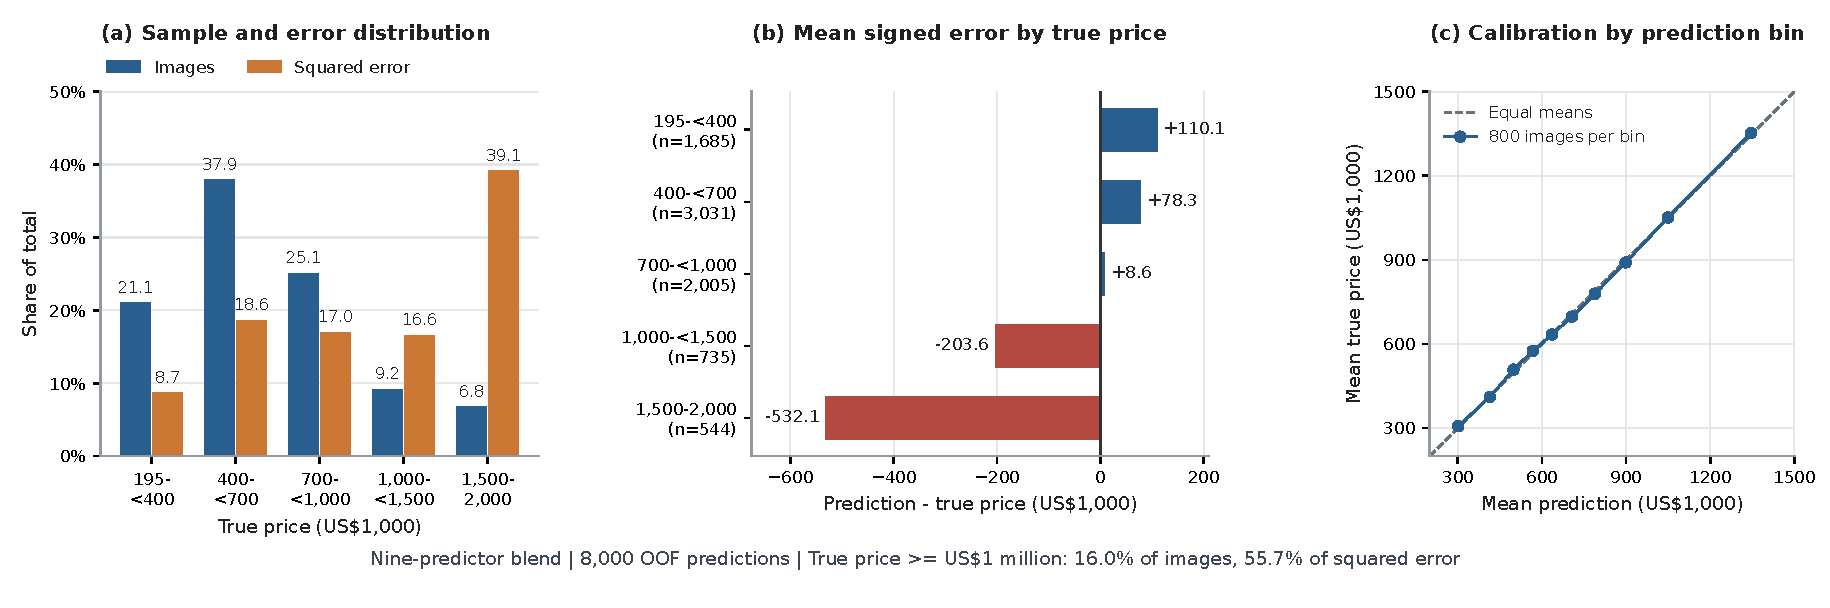
\includegraphics[width=\textwidth]{figure1_ensemble_error_analysis.pdf}
\caption{Error and calibration diagnostics for the final ensemble: (a) sample and squared-error shares by price band; (b) mean prediction bias; and (c) calibration across prediction bins, each holding 800 images. Bin means near the diagonal do not imply accurate estimates for individual images.}
\label{fig:diagnostics}
\end{figure*}

\begin{figure*}[!t]
\centering
\begin{minipage}[t]{0.24\textwidth}
\centering\footnotesize
\textbf{(a) 4244.jpg}\\
\parbox[c][2.1\baselineskip][c]{\linewidth}{\centering\textbf{Near-accurate}}
\par\smallskip
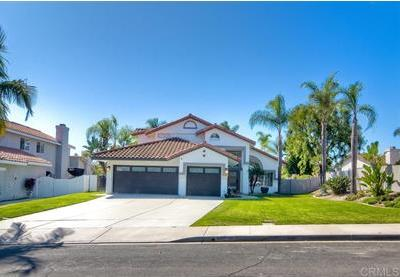
\includegraphics[width=\linewidth,height=32mm,keepaspectratio]{cases/4244.jpg}
\par\smallskip
True: 769.00\\
Predicted: 768.98\\
Error: \ensuremath{-}0.02
\end{minipage}
\hfill
\begin{minipage}[t]{0.24\textwidth}
\centering\footnotesize
\textbf{(b) 2138.jpg}\\
\parbox[c][2.1\baselineskip][c]{\linewidth}{\centering\textbf{Severe underestimate}}
\par\smallskip
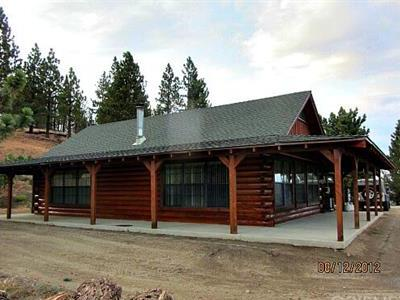
\includegraphics[width=\linewidth,height=32mm,keepaspectratio]{cases/2138.jpg}
\par\smallskip
True: 1,995.00\\
Predicted: 526.61\\
Error: \ensuremath{-}1,468.39
\end{minipage}
\hfill
\begin{minipage}[t]{0.24\textwidth}
\centering\footnotesize
\textbf{(c) 5350.jpg}\\
\parbox[c][2.1\baselineskip][c]{\linewidth}{\centering\textbf{Overestimate}}
\par\smallskip
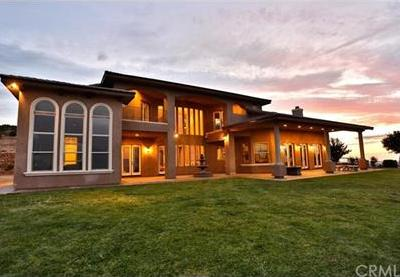
\includegraphics[width=\linewidth,height=32mm,keepaspectratio]{cases/5350.jpg}
\par\smallskip
True: 635.00\\
Predicted: 1,485.39\\
Error: +850.39
\end{minipage}
\hfill
\begin{minipage}[t]{0.24\textwidth}
\centering\footnotesize
\textbf{(d) 2409.jpg}\\
\parbox[c][2.1\baselineskip][c]{\linewidth}{\centering\textbf{Partial tree occlusion}}
\par\smallskip
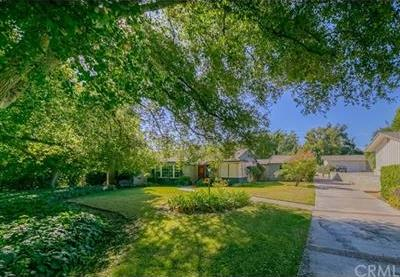
\includegraphics[width=\linewidth,height=32mm,keepaspectratio]{cases/2409.jpg}
\par\smallskip
True: 1,980.00\\
Predicted: 1,176.47\\
Error: \ensuremath{-}803.53
\end{minipage}
\par\medskip{\footnotesize Nine-predictor NNLS blend; OOF predictions; all values in US\$1,000.}
\caption{Four illustrative predictions from the final ensemble, showing a near-accurate estimate, a severe underestimate, an overestimate, and a case with foreground tree occlusion. These are individual examples rather than the overall distribution, and visible image characteristics cannot establish the causes of errors.}
\label{fig:cases}
\end{figure*}

% Typeset from reportdraft.en.md; edit this TeX file for subsequent revisions.

A lower overall error does not mean uniform improvement across price bands. Expensive houses dominate the MSE: the 1,279 images with true prices of at least 1,000 thousand dollars account for 16.0\% of the samples but contribute 55.7\% of the total squared error; there is also a clear direction of bias: the mean ``prediction minus true price'' bias in the 1,500--2,000 thousand dollar band is \ensuremath{-}532.1 thousand dollars, compared with +8.6 thousand dollars in the 700--1,000 band (Fig.~\ref{fig:diagnostics}).


Panels (b) and (c) of Fig.~\ref{fig:diagnostics} group the same predictions in two different ways and should not be read as one statement. Conditioning on the true price, as in (b), makes a predictor with limited information appear biased even when nothing is wrong with it: among houses that happen to be expensive, those the model cannot identify pull the group average down. Panel (c) conditions on the prediction instead, and all ten bins lie close to the diagonal, so the shrinkage in (b) appears calibrated rather than correctable: scaling the high end upwards would move predictions away from the conditional mean that squared error rewards, and the remaining tail error points to how little a photograph reveals about price band.


To further illustrate these MSEs, we show four specific cases from the final model (Fig.~\ref{fig:cases}). The facade in 4244.jpg is clear and its prediction of 768.98 is close to the true 769, which serves as an accurate reference. 2138.jpg is underestimated by 1468, possibly because its wooden exterior walls and sparse surrounding greenery do not reflect its higher true price. 5350.jpg is overestimated by 850, possibly because its tall arched windows, warm lighting and lawn are associated with higher-value houses. In 2409.jpg, there is considerable occlusion from trees in the foreground, which affected the model's judgement of the building's price.


In addition, this study was limited by available compute and runtime, which is also why we mainly used frozen visual features. Fine-tuning the visual encoder, to test whether an adapted representation separates price bands better than a general-purpose one, is therefore the main avenue we were unable to explore.

% !TeX root = ../main.tex

\section{Conclusion}

% Typeset from reportdraft.en.md; edit this TeX file for subsequent revisions.

Taken together, the above comparisons and error analysis show that frozen visual features allow us to estimate house prices usefully even with a limited dataset and compute: on the same five-group split the final ensemble reaches an out-of-fold MSE of 65,278 against 156,686 for predicting the mean training price, and the configuration submitted before the Kaggle leaderboard closed scored 63,952.39 on the test images. In the tested configurations, combining whole-image and local features performed better than using either view alone, while the price-order auxiliary task did not show a clear additional benefit. Expensive houses are still predicted low relative to their true prices, but the calibration diagnostic suggests this reflects how little a photograph reveals about price band rather than a correctable output bias.

% Keep all body text and figures before the bibliography. Only references may
% extend to page five under the course limit; inspect the final PDF after edits.
\FloatBarrier
\bibliographystyle{IEEEtran}
\bibliography{references}
\end{document}
